\chapter{Desarrollo} 
\label{sec:desarrollo}

\section{Arquitectura}

El desarrollo se ha llevado a cabo siguiendo un enfoque basado en microservicios. Comúnmente, las aplicaciones presentan una arquitectura monolítica, esto quiere decir que todos los elementos que se implementan se encuentran contenidos en una aplicación individual. Uno de los principales inconvenientes de este tipo de arquitectura es su rigidez. Solucionar problemas o actualizar la aplicación con nuevas funcionalidades en la aplicación se puede volver difícil y tedioso. 

Para hacer frente a los problemas que supone la arquitectura monolítica, surgió un nuevo tipo de arquitectura de microservicios, donde cada elemento o proceso son independientes y trabajan entre sí para conseguir la funcionalidad que requiere la aplicación. Básicamente, la aplicación se divide en servicios, donde cada uno es un proceso autónomo. La ventaja de este enfoque reside principalmente en este hecho, la independencia de los procesos, puesto que de esta forma es posible introducir cambios sin que ello conlleve ninguna modificación sobre el resto de los servicios. 

En la siguiente figura se comparan ambos tipos de arquitecturas:

\begin{figure}[ht]
	\begin{center}
		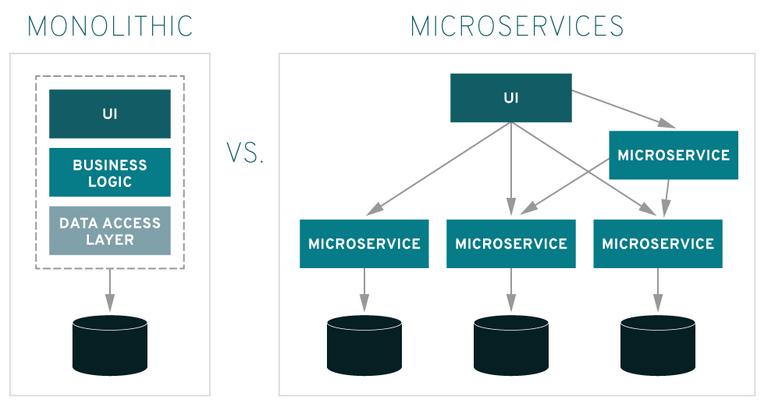
\includegraphics[width = 0.70\textwidth]{Figuras/microservicios.PNG}
	\end{center}
	\caption{\label{fig:microservicios} Comparación de la arquitectura monolítica y de microservicios. Fuente: Red Hat.}
\end{figure}

\newpage

La base del proyecto es una página web construida usando Wordpress. En ella se han incluido una herramienta de análisis de sentimientos y un bot conversacional. Estará conectada a un segmento de Cloud Storage. Aquí se almacenarán los contenidos importados durante su funcionamiento. 

Cuando un comentario es publicado en la página web, se realiza una llamada a la API de la aplicación de análisis de sentimientos para crear su valoración. El servicio encargado de esta acción recupera un comentario de la base de datos y envía una petición a la función adecuada de Natural Language. Por último, devuelve el resultado a Wordpress. Si ocurre algún error en el proceso, creará un nuevo registro en Cloud Logging.

Tanto esta aplicación como Wordpress se despliegan en Cloud Run utilizando contenedores que, previamente, han sido almacenados en Container Registry. Además, ambas usarán la misma instancia de la base de datos en Cloud SQL. 

Por su parte, la implementación del chatbot se ha realizado con Dialogflow, integrándolo en Wordpress mediante una extensión conocida como MyChatbot. Actualmente, no se encuentra conectado con la base de datos, pero se plantea que lo esté en el futuro.

En la siguiente figura se muestra la arquitectura del sistema:

\begin{figure}[ht]
	\begin{center}
		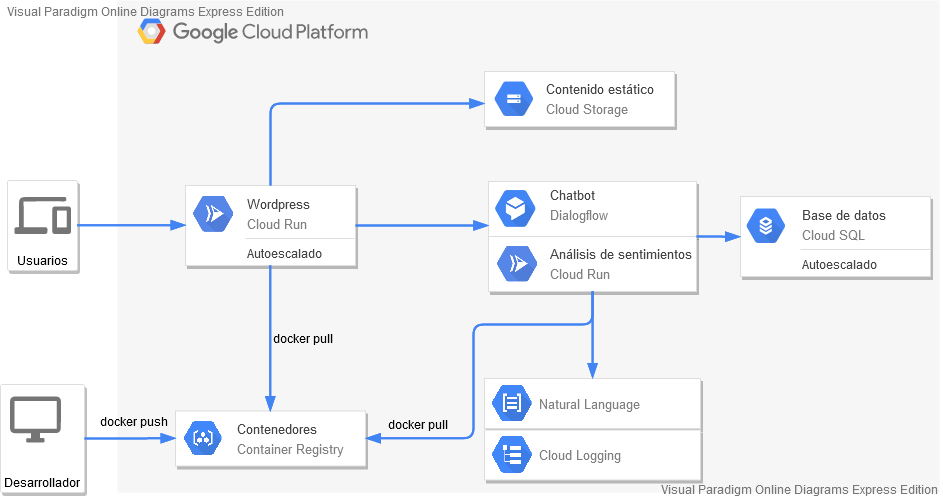
\includegraphics[width = 0.95\textwidth]{Figuras/ArquitecturaV3.png}
	\end{center}
	\caption{\label{fig:systemArchitecture} Arquitectura del sistema}
\end{figure}

\newpage
\section{Implementación}

En esta sección se describe con detalle el proceso que se ha seguido para poner en marcha cada uno de los elementos centrales que componen este proyecto. Se divide en tres subsecciones dedicadas a: página web, análisis de sentimientos y bot conversacional.

\subsection{Página web}

El sitio web se ha desarrollado con Wordpress en un servidor local. Tras finalizar el proceso, se ha introducido en un contenedor y se ha desplegado en la nube. A partir de este momento la página web ya está disponible para los usuarios.

El primer paso consiste en construir el entorno de desarrollo mediante XAMPP. Este programa ya es suficiente para disponer de un servidor web local preparado para alojar una página web. Cómo se puede apreciar en la siguiente figura sólo serán necesarios los módulos de Apache y MySQL:

\begin{figure}[ht]
	\begin{center}
		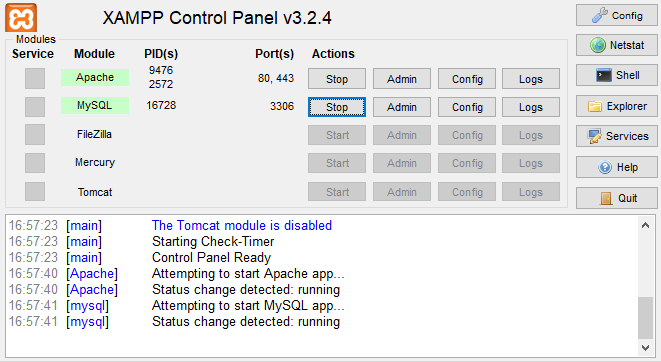
\includegraphics[width = 0.80\textwidth]{Figuras/XAMPP.PNG}
	\end{center}
	\caption{\label{fig:xampp} XAMPP en funcionamiento}
\end{figure}

Para su funcionamiento Wordpress requiere de una base de datos, por lo tanto, el siguiente paso consiste en crear una instancia en el servidor de MySQL de XAMPP. Con este objetivo se utiliza la aplicación de administración phpMyAdmin, que también está incluida en XAMPP. Dicha aplicación se puede visualizar en el navegador desde la dirección \textit{http://localhost/phpmyadmin/}. En la próxima figura se señala la instancia creada:

\begin{figure}[ht]
	\begin{center}
		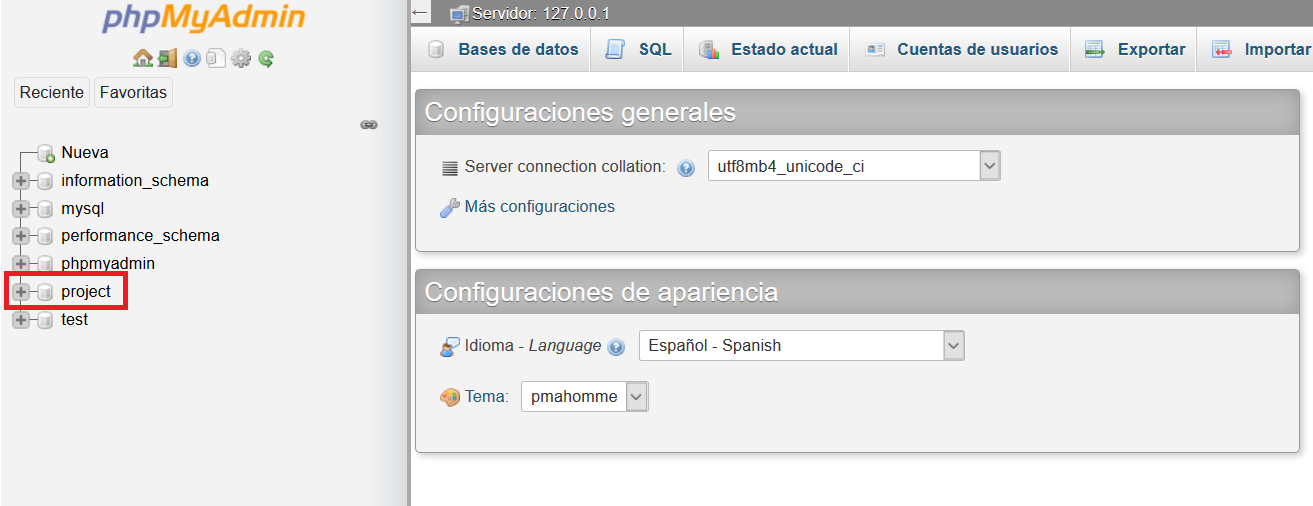
\includegraphics[width=15.93cm, height=6.14 cm, ]{Figuras/phpmyadmin.png}
	\end{center}
	\caption{\label{fig:phpmyadmin} Interfaz de phpMyAdmin}
\end{figure}
\newpage

Una vez hecho esto, se descarga Wordpress desde \url{https://wordpress.org/} y se extrae su contenido en la carpeta htdocs situada dentro del directorio de XAMPP. Esta carpeta es similar a la carpeta public\_html usada por la mayoría de hostings como raíz para la instalación de páginas webs.

Ya sólo queda acceder a la dirección \textit{http://localhost/wordpress/} y seguir los pasos que se van mostrando para finalizar el proceso de instalación.

Si el proceso se ha realizado correctamente se podrá acceder al panel de administración de Wordpress a través de la dirección \textit{localhost/wordpress/wp-admin/}. La siguiente imagen muestra el aspecto de dicho panel:

\begin{figure}[ht]
	\begin{center}
		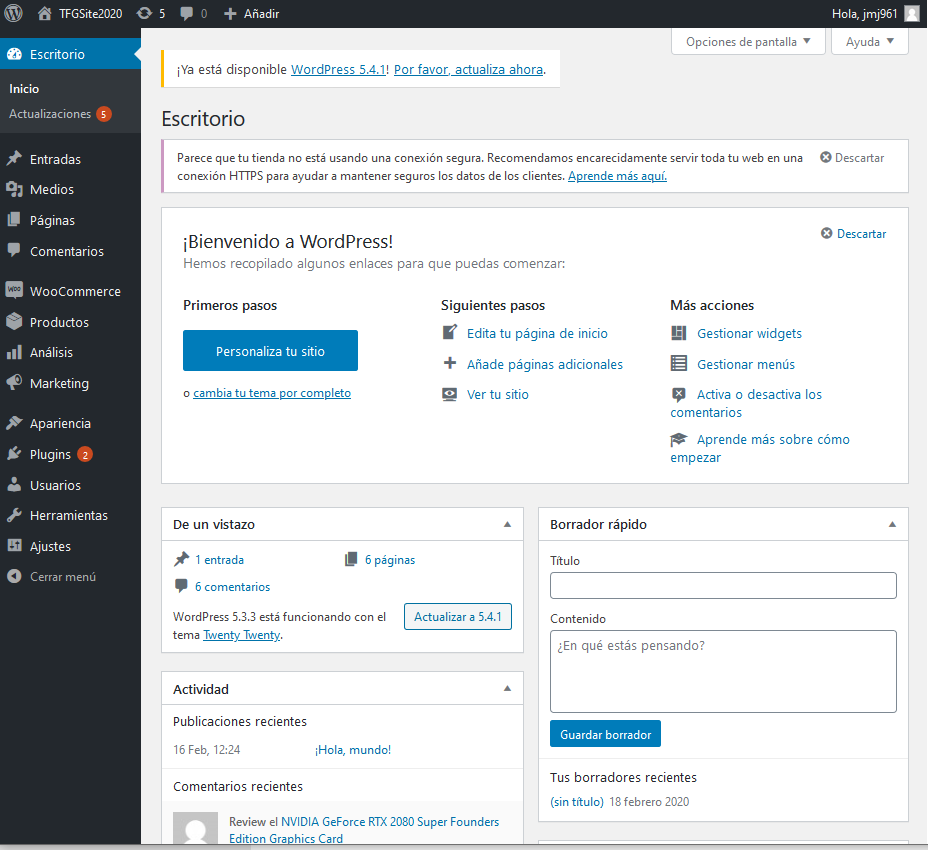
\includegraphics[width = 0.65\textwidth]{Figuras/wpadmin.PNG}
	\end{center}
	\caption{\label{fig:wordpressAdmin} Panel de administración Wordpress}
\end{figure}
\newpage

Ahora, se procede a instalar y configurar los plugins necesarios: WooCommerce, para transformar la página en una tienda de comercio electrónico; MyChatbot, para integrar el bot conversacional, y WP-Stateless, que permitirá otorgar persistencia a los archivos multimedia cargados a la página cuando se realice su despliegue en Cloud Run.

En el siguiente paso se introducen productos y comentarios que serán utilizados más adelante para comprobar el funcionamiento de la aplicación de análisis de sentimientos. Tanto los productos como sus comentarios son ejemplos reales extraídos de Amazon y PcComponentes.

Por último, se modificará el diseño del sitio con la intención de que resulte más atractivo a los usuarios. Con esta idea, se ha utilizado la versión gratuita de la extensión Elementor, que simplifica considerablemente dicha tarea. La explicación de este proceso se va a obviar por considerarse que queda fuera a los objetivos de este trabajo. La siguiente imagen muestra uno de los productos ofertados en la página web:

\begin{figure}[ht]
	\begin{center}
		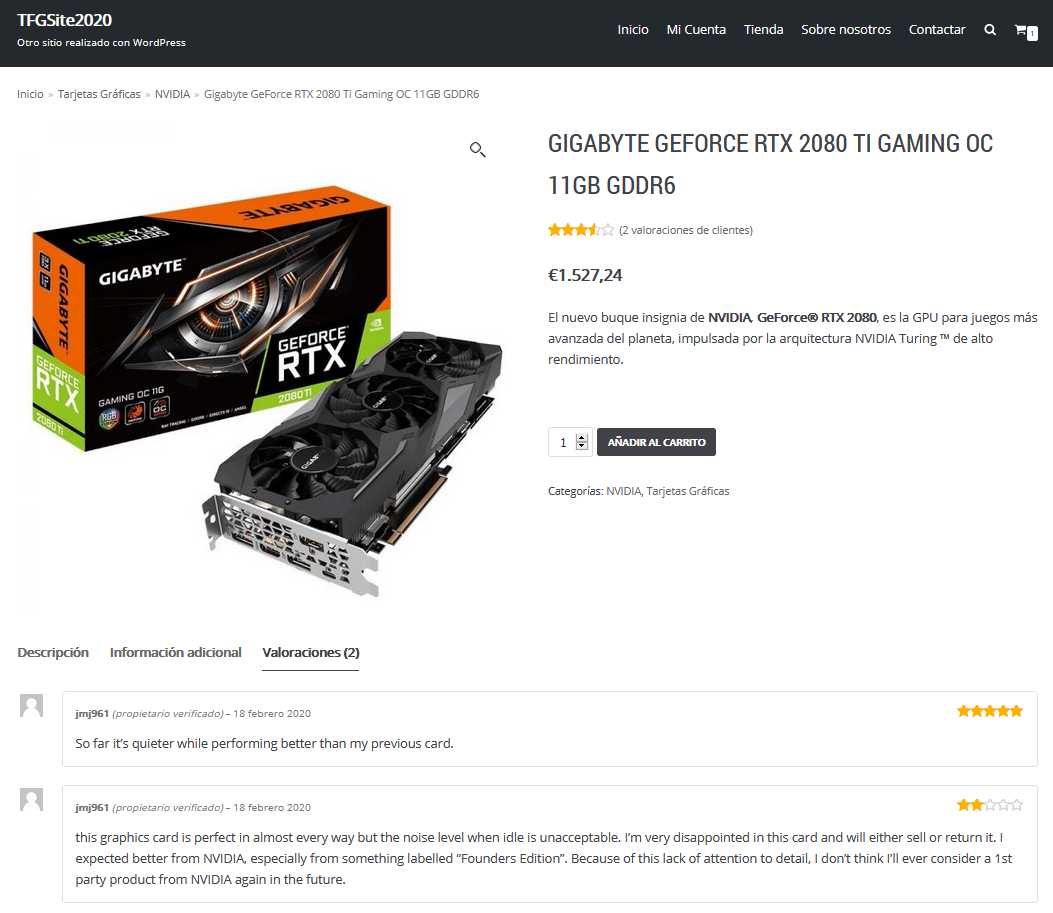
\includegraphics[width = 0.80\textwidth]{Figuras/tiendaWordpress.PNG}
	\end{center}
	\caption{\label{fig:tienda} Tarjeta gráfica ofertada en la página web}
\end{figure}
\newpage

\subsection{Análisis de sentimientos}

El análisis de opiniones de los comentarios que los usuarios publican en el sitio web se realiza mediante una aplicación desarrollada en GoLang. Ésta actúa como envoltorio del servicio de procesamiento del lenguaje natural ofrecido por Google a través de su nube. Todo el código de la aplicación está disponible en \url{https://github.com/jo4nymj/sentiment-analysis}. El proyecto presenta la siguiente estructura:
\begin{itemize}
    \item \textbf{Paquetes}
    \begin{itemize}
        \item \textbf{database}. Establece la conexión con la base de datos. Se ha optado por implementar un patrón de diseño Singleton para que exista una única instancia de la base de datos a la que se accede a través de un punto de acceso global. Para establecer una conexión con la base de datos desde otro paquete basta con hacer referencia a la variable \textit{Instance}. 
        
        \begin{lstlisting}[caption= Singleton]
        var Instance *Connection
        func init() {
        	if Instance == nil {
        		Instance = GetMySQLDB() // Devuelve &Connection{Conn: db}
        	}
        }
        type Connection struct {
        	Conn *sql.DB
        }
        \end{lstlisting}
        
        En Go, la función init() se ejecuta antes que cualquier otro fragmento del código del paquete donde se incluya la función. Por tanto, se ejecutará en el momento en el que se importe el paquete.
        
        \item \textbf{config}. Aquí se incluyen las variables de configuración relacionadas con la conexión a la BBDD y a la generación del token de seguridad que se utiliza en las peticiones. Se comprueba si el entorno en el que se está ejecutando la aplicación es local o producción y, en función de ello se asignan valores a las variables.
        
        \item \textbf{logger}. Crea e inicializa un cliente para establecer la comunicación con el servicio de Cloud Logging. Del mismo modo, implementa las funciones que se utilizarán para realizar el envío de los registros: \textit{Print} y \textit{Error}.
        
        \item \textbf{models}. Es necesario un modelo para los comentarios y otro para los productos. En Go no existen las clases, pero se puede conseguir que los structs utilizados para crear los modelos actúen como tal asignándoles métodos. Seguidamente se expone el diagrama de clases:
        
        \begin{figure}[ht]
        	\begin{center}
        		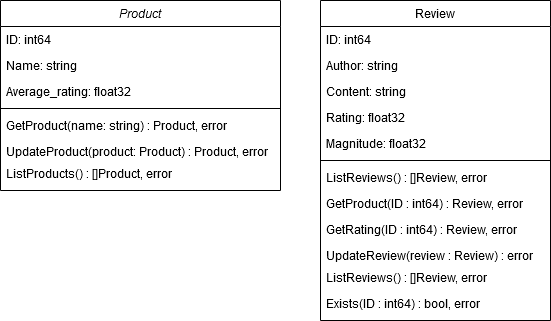
\includegraphics[width=0.80\textwidth]{Figuras/DiagramaClases.png}
        	\end{center}
        	\caption{\label{fig:classDiagram} Diagrama de clases}
        \end{figure}
        
        \newpage
        
        Ha sido necesario introducir modificaciones en el modelo de comentario con el que trabaja WooCommerce. De forma predeterminada, se crean dos entradas asociadas a un comentario en la tabla \textit{wp\_commentmeta}. Una de estas entradas sirve para identificar si un comentario está verificado, si no lo está, éste no será mostrado a los usuarios de la página web. La otra entrada es utilizada por Wordpress para almacenar la valoración que un usuario introduce junto a su comentario (\textit{meta\_value}). Por tanto, como Google NLP devuelve dos valores (puntuación y magnitud), se ha decidido reutilizar el campo de \textit{meta\_value} para asignar la puntuación y añadir una nueva columna para la magnitud. En la siguiente figura se muestra parte del contenido de la tabla \textit{wp\_commentmeta}:
        
        \begin{figure}[ht]
        	\begin{center}
        		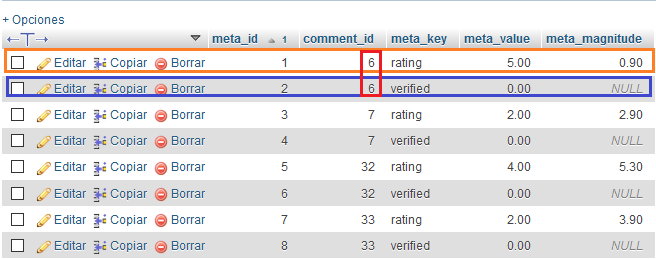
\includegraphics[width = 0.95\textwidth]{Figuras/wp_commentmeta.PNG}
        	\end{center}
        	\caption{\label{fig:commentmeta} Tabla wp\_commentmeta}
        \end{figure}
        
        \newpage 
        
        En naranja se ha señalado la entrada correspondiente a la evaluación del comentario y en azul la que corresponde al estado de verificación. Se puede identificar claramente a qué corresponde cada entrada si se observa el valor de la columna \textit{meta\_key}. En rojo se resalta que ambas entradas se refieren al mismo comentario puesto que comparten el valor de \textit{comment\_id}.
        
        \item \textbf{repository}. Aquí se definen los métodos asociados a los modelos donde se realizan operaciones sobre la base de datos como extraer, actualizar o ingresar datos.
        
        \item \textbf{services}. Se han implementado métodos que permiten interactuar con los productos y sus comentarios para poder crear  y actualizar los modelos, así como recuperar información sobre ellos. 
        
        En relación a los productos se han implementado dos métodos:
        \begin{itemize}
            \item \textbf{Obtener un producto}. Dado el nombre de un producto permite obtener de la base de datos su información.
            \item \textbf{Actualizar un producto}. A partir del nombre de un producto, fuerza la actualización de su puntuación. Para ello, recorre sus comentarios y obtiene la media de puntuación. De forma normal, Wordpress actualiza la puntuación del producto cada vez que se evalúa una nueva opinión. Aún así, en algunas ocasiones este proceso puede presentar fallos y no actualizar correctamente la información, por lo que se ha visto conveniente implementar este método para atajar posibles problemas.
        \end{itemize}
        
        En cuanto a las opiniones o comentarios se han definido los siguientes métodos:
        \begin{itemize}
            \item \textbf{Listar opiniones}. Dado el id de un producto se listan todos sus comentarios, conteniendo la información sobre su valoración.
            \item \textbf{Crear valoración de una opinión}. A partir del identificador de un comentario, extrae su información de la base de datos; si aún no ha sido evaluado, realiza una llamada a la API de Google para hacerlo y almacena el resultado.
            \item \textbf{Actualizar opiniones}. Fuerza la llamada a la API de Google para actualizar los valores de puntuación y magnitud de un comentario específico.
        \end{itemize}
        
        \newpage
        
        A continuación, se muestra un diagrama que modela las interacciones con la API:
        
         \begin{figure}[ht]
        	\begin{center}
        		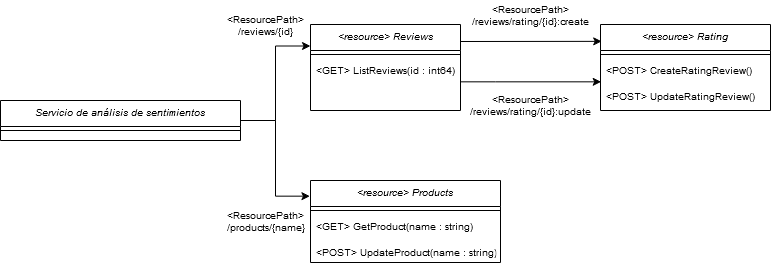
\includegraphics[width = 0.95\textwidth]{Figuras/DiagramaAPI.png}
        	\end{center}
        	\caption{\label{fig:modelAPI} Modelo de la API}
        \end{figure}
    \end{itemize}
    \item \textbf{Ficheros}
     \begin{itemize}
        \item \textbf{main}. En este fichero se establecen las URLs de acceso a cada uno de los servicios y el puerto a través del cual se realizará la comunicación.
        \item \textbf{go.mod}. Incluye los módulos con los que el proyecto presenta dependencias.
        \item \textbf{go.sum}. En este fichero se encuentran los hashes criptográficos de las versiones específicas de los módulos.
        \item \textbf{Dockerfile}. Contiene las instrucciones para crear la imagen del contenedor. Su implementación se explicará más adelante en la subsección 6.3.2.
    \end{itemize}
\end{itemize}

Tras haber expuesto de manera general la estructura del proyecto y haber hablado brevemente sobre la función de cada uno de sus componentes, resulta conveniente tratar con más profundidad el método destinado a crear valoraciones de un comentario. 

Hay algo que se debe tener en cuenta para entender la manera en la que se ha construido este método. Como ya se explicó anteriormente en la subsección 4.1.1, por defecto se requiere al usuario introducir una valoración junto con su comentario a través de un componente gráfico con forma de estrellas. Esta funcionalidad ha sido modificada para que no sea el usuario quien introduzca dicha valoración, sino que ésta venga dada por la evaluación de Google NLP. El comentario será almacenado en un primer momento en la tabla \textit{wp\_comment} sin valoración, por lo tanto la tabla \textit{wp\_commentmeta} no contará con una entrada destinada a su puntuación. Será el método \textit{CreateRatingReview} el encargado de crear dicha entrada en la tabla de \textit{wp\_commentmeta}. Seguidamente se muestra el diagrama de secuencia que modela el proceso para crear una valoración:

\begin{figure}[ht]
	\begin{center}
		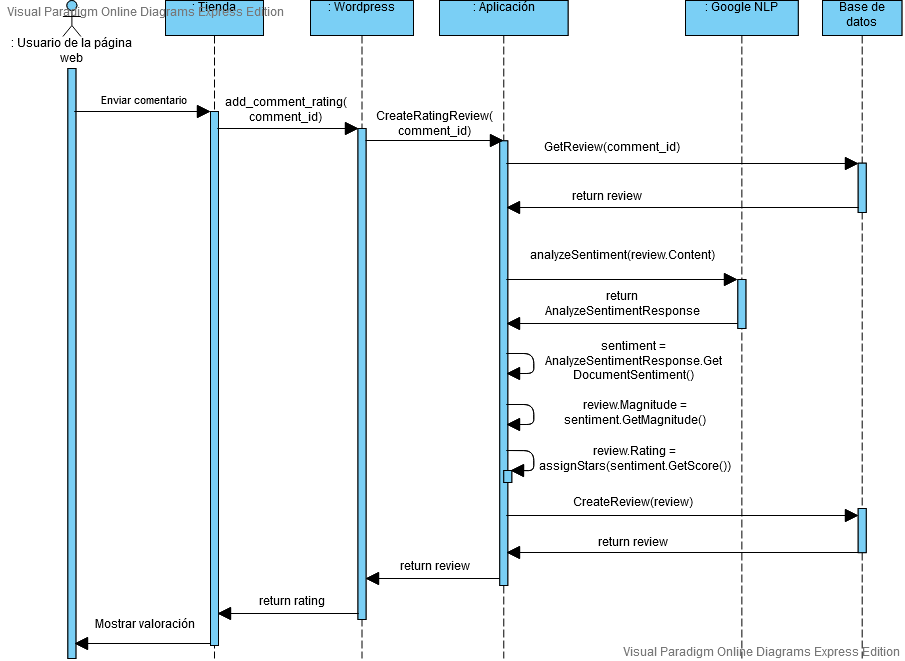
\includegraphics[width = 1\textwidth]{Figuras/DiagramaSecuencia.png}
	\end{center}
	\caption{\label{fig:sequenceDiagram} Diagrama de secuencia CreateRatingReview}
\end{figure}
\newpage
Tras esto se procede a presentar la implementación del mismo:
\begin{lstlisting}[caption= M\'etodo para crear una valoraci\'on de un comentario]
func CreateRatingReview(w http.ResponseWriter, r *http.Request) {
	reviewModel := repository.ReviewModel{
		Db: database.Instance,
	}
	reviewID, err := strconv.ParseInt((mux.Vars(r)["id"]), 10, 64)
	if err != nil {
		logger.Error("Failed to parse the ID of the review, %v", err)
		utilities.StatusInternalServerError(w, r)
	}
	exists, err := reviewModel.Exists(reviewID)
	if err != nil {
		logger.Error("Failed to retrieve the review from the database, %v", err)
		utilities.StatusBadRequest(w, r, "")
	}
	if exists {
		utilities.StatusBadRequest(w, r, "Review already exists")
		return
	}
	review, err := reviewModel.GetReview(reviewID)
	if err != nil {
		logger.Error("Failed to retrieve the review from the database, %v", err)
		utilities.StatusBadRequest(w, r, "")
	}
	if err := analyze(&review); err != nil {
		logger.Error("Failed to analyze the review, %v", err)
		utilities.StatusInternalServerError(w, r)
	}
	if err := reviewModel.CreateReview(review); err != nil {
		logger.Error("Failed to create review: %v", err)
		utilities.StatusBadRequest(w, r, "")
	}
	json.NewEncoder(w).Encode(review)
}
\end{lstlisting}

En primer lugar se extrae el identificador del comentario incluido en la petición. A partir de este parámetro se comprueba si el comentario ya tiene una valoración registrada, en cuyo caso se responde a la petición con un estado 400, si no, se llama al método \textit{GetReview()} para obtener su entrada de la tabla \textit{wp\_comment}.

Posteriormente se procede a invocar a la función \textit{analyze()} dónde será evaluado el contenido del comentario. Esta función se ha construido de la siguiente forma:

\begin{lstlisting}[caption= Funci\'on que envuelve la llamada a la API de NLP]
func analyze(review *models.Review) error {
	ctx := context.Background()
	client, err := language.NewClient(ctx)
	if err != nil {
		return err
	}
	v, err := analyzeSentiment(ctx, client, review.Content)
	if err != nil {
		return err
	}
	sentiment := v.GetDocumentSentiment()
	review.Rating = assignStars(sentiment.GetScore())
	review.Magnitude = sentiment.GetMagnitude()

	return nil
}
\end{lstlisting}

La función comienza por crear un contexto y un cliente para establecer la comunicación con el servicio de destino. Un contexto en Golang es una forma de transmitir información entre una API y los procesos, información como: plazos máximos (deadlines), señales de cancelación y otros valores de alcance de la solicitud. 

Después se invoca a la API NLP desde la función \textit{analyzeSentiment()} pasando como parámetros un contexto, un cliente y el texto a evaluar. En el siguiente listado se puede apreciar como la función utiliza el cliente para invocar el servicio escogido de NLP y construye una petición con el texto a evaluar. 

\begin{lstlisting}[caption= Llamada a la API de NLP]
func analyzeSentiment(ctx context.Context, client *language.Client, text   string) (*languagepb.AnalyzeSentimentResponse, error) {
    return client.AnalyzeSentiment(ctx, &languagepb.AnalyzeSentimentRequest{
	Document: &languagepb.Document{
		Source: &languagepb.Document_Content{
			Content: text,
		},
		Type: languagepb.Document_PLAIN_TEXT,
	},
    })
}
\end{lstlisting}

La respuesta proporcionada por el servicio tiene la siguiente estructura:

\begin{lstlisting}[caption= Respuesta del servicio de NLP]
type AnalyzeSentimentResponse struct {
    // El sentimiento general del texto introducido
    DocumentSentiment *Sentiment
    // El lenguaje del texto, coincide con el especificado en la petición.
    // Si no fue especificado, es detectado automáticamente.
    Language string
    // El sentimiento de cada una de las frases del texto.
    Sentences []*Sentence
}
\end{lstlisting}
Para exponer este servicio, Google ha hecho uso de gRPC un proyecto open source desarrollado por ellos mismos. Está construido a partir del protocolo RPC (remote procedure call), permitiendo de este modo llamar desde una aplicación cliente a un servicio que se encuentre definido en un servidor como si se invocara a un procedimiento local. De forma simplificada la idea consiste en definir servicios compuestos por una serie de métodos RPC donde se especifican los mensajes de entrada que reciben y los mensajes de salida que generan.

\begin{figure}[ht]
\begin{center}
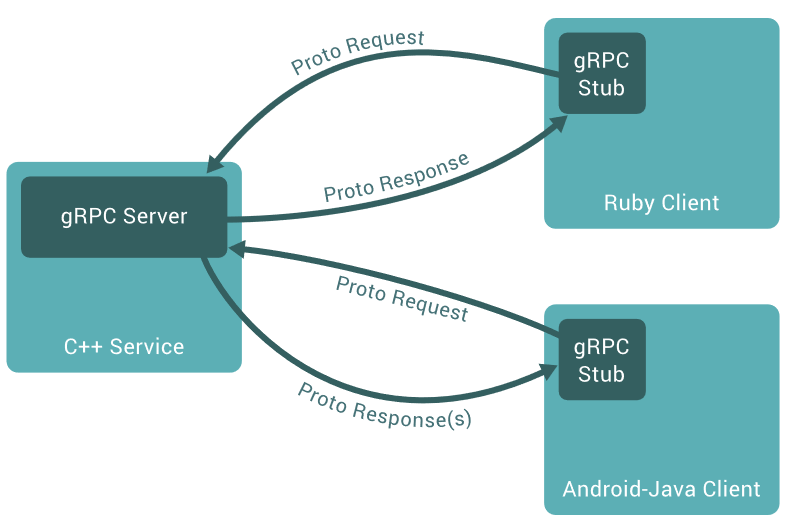
\includegraphics[width = 0.80\textwidth]{Figuras/gRPC.PNG}
\end{center}
\caption{\label{fig:grpc} Sistema gRPC. Fuente: gRPC.io.}
\end{figure}

Por defecto gPRC hace uso de Protocol Buffers o Protobuf para definir los servicios y los mensajes. Se trata un formato binario creado por Google para la serialización de información entre servicios. Actualmente, el formato más usado para este objetivo es JSON, sin embargo, Protobuf ofrece un mejor rendimiento, una mejor capacidad de mantenimiento y un tamaño más pequeño. Google proporciona un generador de código para los principales lenguajes de programación como, JavaScript, Java, PHP, C\#, Ruby, Objective C, Python, C++ y Go. Además Protobuf dispone de más tipos de datos que JSON, como enumeraciones y métodos.

Por este motivo la función \textit{analyzeSentiment} contiene una referencia a \textit{*languagepb}, que no es más que la definición del servicio haciendo uso de Protobuf.

Antes de almacenar el resultado de la petición se discretiza el campo Score (la puntuación) mediante la función \textit{assignStars()}. Esta función consiste en un switch donde se establece la cantidad de estrellas que corresponde  a un intervalo decimal específico, como se puede observar a continuación:

\begin{lstlisting}[caption= Funci\'on para discretizar la puntuaci\'on de una valoraci\'on]
func assignStars(rating float32) float32 {
	switch {
	case rating >= -1.0 && rating < -0.7:
		return 1.0
	case rating >= -0.7 && rating < -0.3:
		return 2.0
	case rating >= -0.3 && rating < 0.3:
		return 3.0
	case rating >= 0.3 && rating < 0.7:
		return 4.0
	case rating >= 0.7 && rating <= 1.0:
		return 5.0
	default:
		return 0.0
	}
}
\end{lstlisting}
    
Finalmente, se invoca al método CreateReview que se encarga de insertar la valoración del comentario en la tabla de \textit{wp\_commentmeta}.

\newpage

\subsubsection{Integración}

Se deben realizar las siguientes modificaciones en el backend de Wordpress:
\begin{enumerate}
\item \textbf{No requerir una valoración}. Se elimina el código existente desde la línea 122 a la 133 del fichero \textit{single-product-reviews.php}. De esta forma, ya no se exige al usuario introducir una valoración y tampoco se muestra el campo para hacerlo cuando éste escribe el comentario. El fragmento de código descartado es:

     \begin{lstlisting}[caption= No requerir una valoraci\'on al introducir un comentario]
if ( wc_review_ratings_enabled() ) {
	$comment_form['comment_field'] = '<div class="comment-form-rating"><label for="rating">' . esc_html__( 'Your rating', 'woocommerce' ) . '</label><select name="rating" id="rating" required>
		<option value="">' . esc_html__( 'Rate&hellip;', 'woocommerce' ) .'</option>
		<option value="5">' . esc_html__( 'Perfect', 'woocommerce' ) . '</option>
		<option value="4">' . esc_html__( 'Good', 'woocommerce' ) . '</option>
		<option value="3">' . esc_html__( 'Average', 'woocommerce' ) . '</option>
		<option value="2">' . esc_html__( 'Not that bad', 'woocommerce' ).'</option>
		<option value="1">' . esc_html__( 'Very poor', 'woocommerce' ) . '</option>
	</select></div>';
}
    \end{lstlisting}
\item  \textbf{Invocar al servicio de análisis de sentimientos}. Las valoraciones de los comentarios son añadidas por la función \textit{add\_comment\_rating()} que se encuentra en el fichero \textit{class-wc-comments.php} en la línea 161. Al principio de esta función se debe realizar una llamada al método de la API encargado de crear la valoración de un comentario, tal y como se muestra a continuación: 
    \begin{lstlisting}[caption= Llamar desde Wordpress al servicio de an\'alisis de sentimientos]
        $sentiment_api_url = 'http://localhost:5002/reviews/rating/' . $comment_id . ':create';
		$headers = array (
			'Authorization' => 'Bearer ' . getenv('TOKEN')
		);
		$args = array(
			'method' => 'POST',
			'headers' => $headers,
		);
		$response = wp_remote_request( $sentiment_api_url, $args );
    \end{lstlisting}
\end{enumerate}

Se realizará una petición de tipo POST a la dirección expuesta incluyendo en la cabecera un token de verificación que autorice la llamada a dicho servicio. Sólo se requerirá autorización al usuario de la API cuando se despliegue la aplicación en la nube, por lo que en local este parámetro será ignorado. Es importante sustituir la URL actual por la que corresponda cuando la aplicación sea desplegada.

\newpage

\subsection{Bot conversacional}

Desarrollar un bot conversacional para automatizar un proceso de negocio complejo, como el servicio de atención al cliente, no es una tarea sencilla. Las conversaciones poco comunes son muy difíciles de estructurar, ya que necesitan de un árbol de decisiones con cientos de declaraciones condicionales y encadenadas.

Por ejemplo, si se desea modelar una conversación que cuenta con 2 preguntas y 3 posibles respuestas harán falta 12 intents. Sin embargo, para modelar una conversación más realista, considerando un total de 10 preguntas con 2 posibles respuestas, supondría un total de 2047 intents. Aunque no sea necesario alcanzar ese número porque la conversación no va a tomar todas las posibles opciones, aún es necesaria una cantidad importante de intents.

Este trabajo tan sólo pretende mostrar el potencial que tiene la implementación de un bot conversacional en una tienda de comercio electrónico. Por tanto, se ha optado por implementar un bot para modelar procesos sencillos tales como la búsqueda de productos, ofrecer recomendaciones y resolver preguntas específicas. 

Al estrechar el dominio de la conversación limitando las opciones del cliente, se consigue reducir la complejidad de implementación, pero el usuario perderá la sensación de estar hablando con otra persona.

\subsubsection{Flujos de conversación}

En primer lugar, hay que definir los flujos de conversación que puede generar el usuario final. En este caso se ha identificado cada flujo de conversación con una de las funcionalidades del chatbot. A la hora de diseñar el trascurso de la conversación se han mezclado dos estilos: en algunos momentos el agente simplemente solicita al usuario final que seleccione una de las opciones que se le presentan mediante el uso de botones, mientras que en otros, se deja libertad al usuario para introducir la entrada de texto que considere oportuna.

A continuación, se va a describir cada uno de estos flujos adjuntando un diagrama que sirva como ejemplo para ilustrar la conversación entre el usuario (naranja) y el agente (azul). Las frases introducidas por el usuario que aparecen entren comillas indican entradas variables, es decir, se espera que el usuario pueda introducir cualquier entrada de texto. Por el contrario, cuando no aparece entrecomillada indica que la entrada se realiza a partir de una selección presentada por el agente (pulsar el botón correspondiente a la opción).

\begin{itemize}
    \item \textbf{Buscar un producto}. Su finalidad es que el usuario obtenga un enlace al catálogo de productos deseado. El agente le preguntará por el tipo de producto y la marca del mismo. A partir de las opciones escogidas por el usuario, el agente le responderá con un enlace al catálogo de dichos productos.
    \begin{figure}
    \begin{center}
    	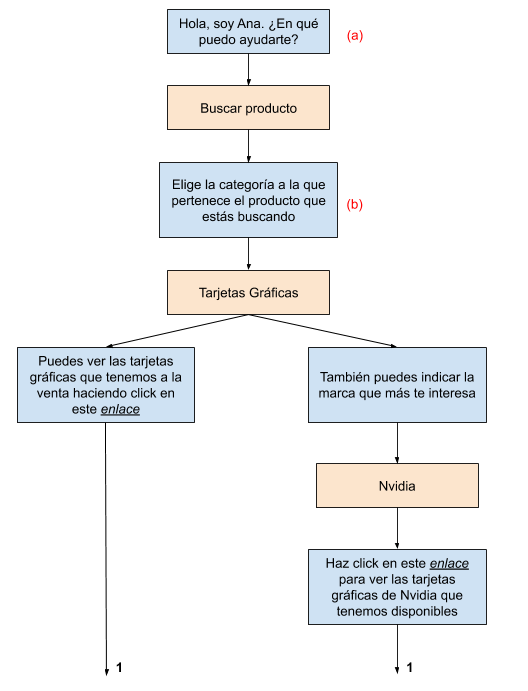
\includegraphics[width = 0.60\textwidth]{Figuras/Buscar producto (1).png}
    	\caption{\label{fig:buscarProducto1} Flujo de conversación para Buscar un producto. Parte I}
    	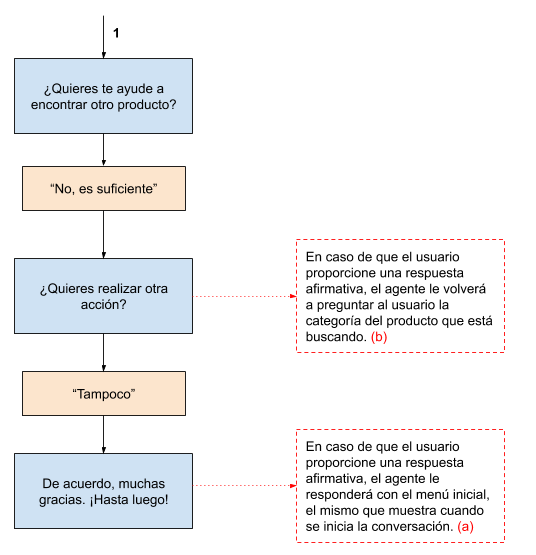
\includegraphics[width = 0.60\textwidth]{Figuras/Buscar producto (2).png}
    	\caption{\label{fig:buscarProducto2} Flujo de conversación para Buscar un producto. Parte II}
	\end{center}
    \end{figure}
    
    \newpage

    \item \textbf{Pedir una recomendación}. El agente pide al usuario que seleccione el tipo de producto y su marca, y según esta información recomienda el producto mejor valorado por los clientes que cumpla con los requisitos establecidos. 
    
    \begin{figure}
    	\begin{center}
    		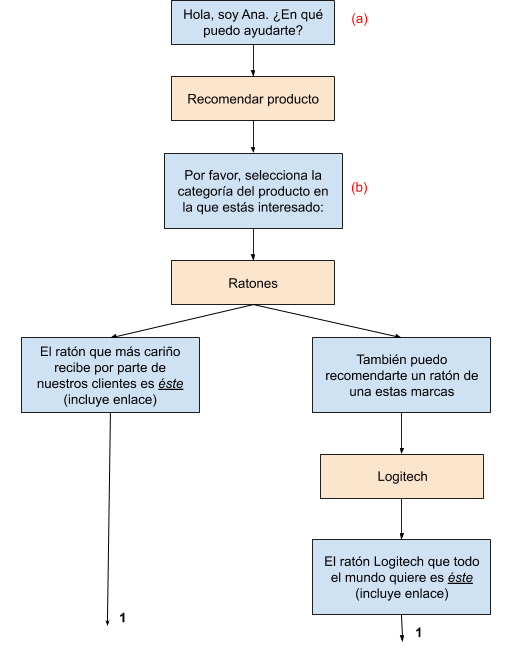
\includegraphics[width = 0.60\textwidth]{Figuras/Recomendar producto (1).png}
    		\caption{\label{fig:recomendarProducto1} Flujo de conversación para Pedir una recomendación. Parte I}
    		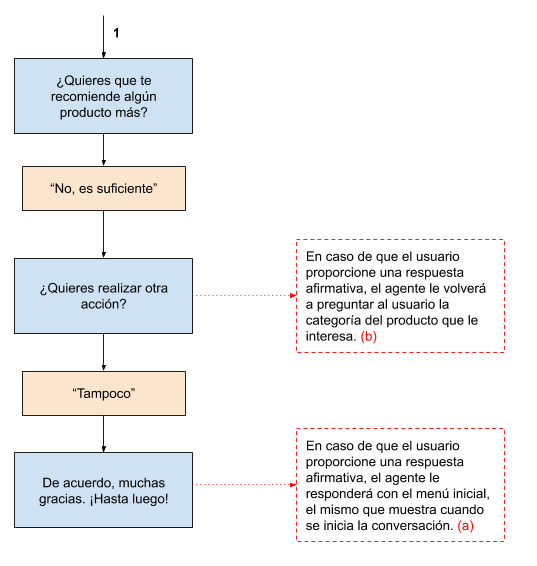
\includegraphics[width = 0.60\textwidth]{Figuras/Recomendar producto (2).png}
    		\caption{\label{fig:recomendarProducto2} Flujo de conversación para Pedir una recomendación. Parte II}
    	\end{center}
    \end{figure}
\newpage
    \item \textbf{Pedir un agente humano}. Si el usuario desea ponerse en contacto con un empleado de la empresa puede iniciar este flujo de conversación. El agente le proporcionará un enlace al formulario para contactar con el servicio de atención al cliente.
    \begin{figure}[ht]
    	\begin{center}
    		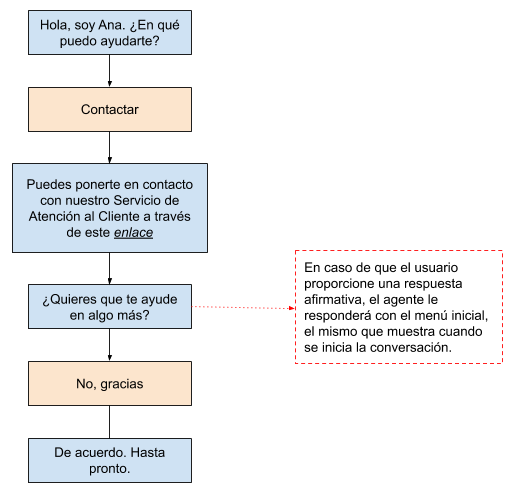
\includegraphics[width = 0.60\textwidth]{Figuras/Contactar.png}
    	\end{center}
	\caption{\label{fig:contactarAgente} Flujo de conversación para Solicitar un agente humano}
    \end{figure}
    
    \item \textbf{Realizar una consulta genérica}. El usuario puede realizar diversas preguntas relacionadas con el servicio de atención al cliente. Suelen estar resueltas en el apartado de preguntas frecuentes que se puede encontrar en la mayoría de tiendas online. Por ejemplo: preguntar acerca de las medidas que la empresa ha tomado ante el coronavirus, garantías, plazos de entrega, medios de pago, etc.
    \begin{figure}[ht]
    	\begin{center}
    		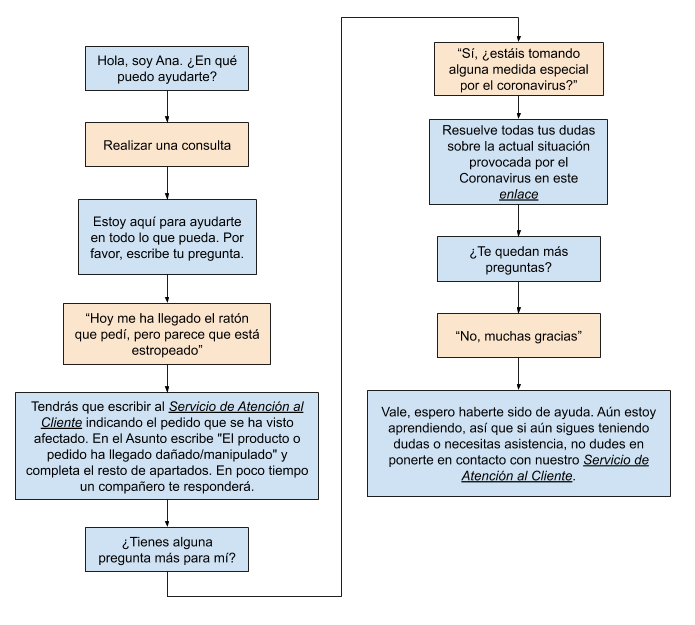
\includegraphics[width = 0.80\textwidth]{Figuras/Realizar consulta.png}
    	\end{center}
	\caption{\label{fig:realizarConsulta} Flujo de conversación para Realizar una consulta genérica}
    \end{figure}

\newpage
    
    \item \textbf{Comprobar el estado del pedido}. El agente pregunta al usuario cuál es el número del pedido sobre el que desea realizar la consulta. En este proyecto, el agente simplemente ofrece una respuesta predefinida, aunque en el futuro sería conveniente que se ligara esta pregunta a una consulta realizada sobre la base de datos. El número de pedido se ha definido como una entidad, por lo que el agente es capaz de extraerlo de la entrada de datos y almacenarlo en un variable.
    \begin{figure}[ht]
    	\begin{center}
    		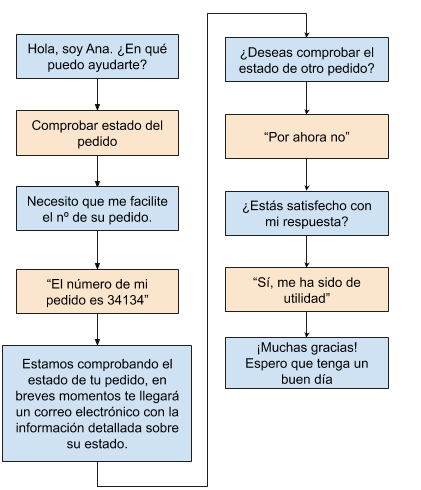
\includegraphics[width = 0.60\textwidth]{Figuras/Comprobar estado del pedido.png}
    	\end{center}
	\caption{\label{fig:estadoPedido} Flujo de conversación Comprobar estado del pedido}
    \end{figure}
\newpage

\end{itemize}

\subsubsection{Intents}

Se han creado diferentes intents para soportar cada flujo de conversación que se puede dar entre el agente y el usuario. Estas intenciones tienen que ver con el saludo, la búsqueda y recomendación de productos, conocer el estado de un pedido y el servicio de atención al cliente. En la siguiente figura se pueden observar los intents principales:

\begin{figure}[ht]
	\begin{center}
		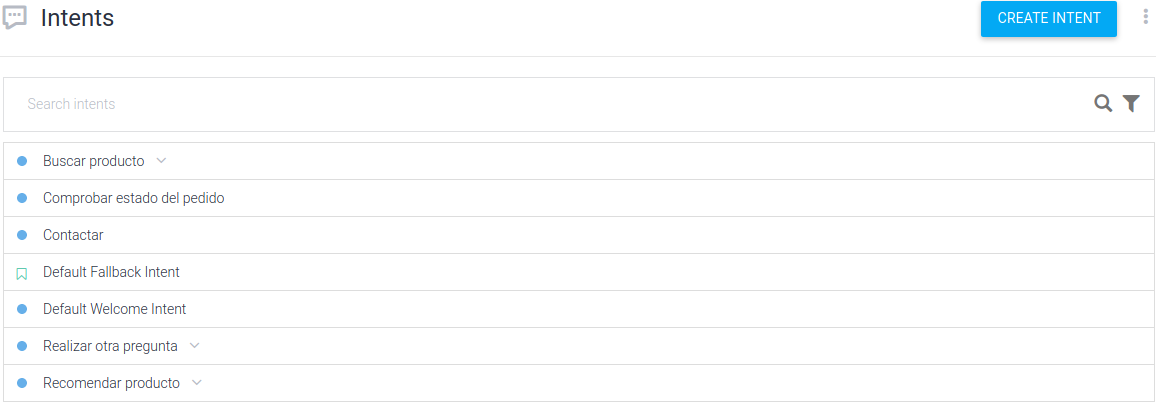
\includegraphics[width = 0.93\textwidth]{Figuras/intents.png}
	\end{center}
	\caption{\label{fig:intenciones} Intents implementados}
\end{figure}
\newpage


Para cada intent se han especificado diferentes frases de entrenamiento que actúan como ejemplo de posibles frases que los usuarios podrían escribir. Estas frases ayudan al aprendizaje del motor de lenguaje de Dialogflow. El agente no sólo intentará establecer una coincidencia con las frases registradas aquí, sino que el motor de lenguaje está continuamente aprendiendo y a partir de las frases introducidas tendrá en cuenta otras opciones. Todo esto ayuda a que el agente comprenda mejor la intención del usuario y establezca una coincidencia con el intent más apropiado. En la siguiente imagen se presentan las frases de entrenamiento usadas para configurar el intent "Realizar otra pregunta - paquete manipulado":

\begin{figure}[ht]
	\begin{center}
		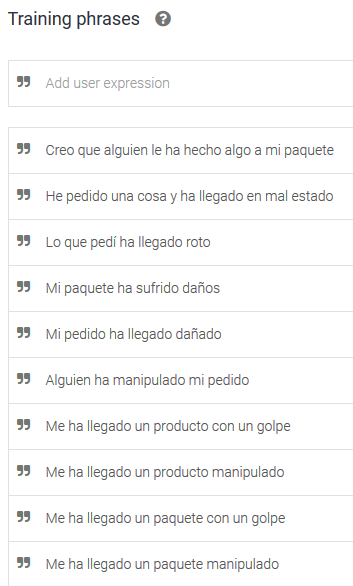
\includegraphics[width = 0.40\textwidth]{Figuras/trainingPhrases.PNG}
	\end{center}
	\caption{\label{fig:frasesEntrenamiento} Frases de entrenamiento configuradas}
\end{figure}
\newpage

Cuando el usuario realice una petición, el agente buscará la frase más parecida entre todas estas frases de entrenamiento y establecerá una coincidencia con el intent al que pertenezca dicha frase. Siguiendo con el ejemplo anterior, cuando el agente establece una coincidencia con el intent "Realizar otra pregunta - paquete manipulado" responderá como se muestra a continuación:

\begin{figure}[ht]
	\begin{center}
		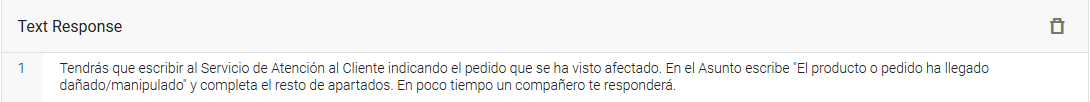
\includegraphics[width = 0.95\textwidth]{Figuras/intentResponse.PNG}
	\end{center}
	\caption{\label{fig:respuesta} Respuesta configurada}
\end{figure}

Al introducir las frases de entrenamiento, se pueden asignar una palabra o conjunto de ellas a un tipo de entidad. Estas palabras son extraídas en forma de parámetros o variables que se pueden utilizar para realizar alguna lógica u ofrecer mejores respuestas a los usuarios. Para ilustrar el funcionamiento de los parámetros, se pone como ejemplo el intent "Comprobar el estado del pedido" donde el agente recibe una petición por parte del usuario para comprobar la situación de su pedido. Cuando el agente procesa la petición, busca el número de pedido que previamente se ha establecido como un valor requerido, y si no lo encuentra se lo pedirá al cliente antes de ofrecerle la información sobre su pedido. En la siguiente imagen aparecen en color verde los caracteres que se han identificado como entidad "PedidoID":

\begin{figure}[ht]
	\begin{center}
		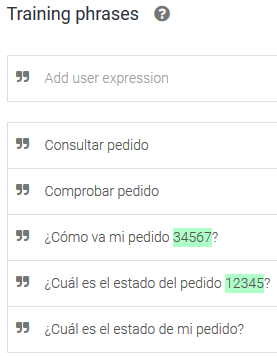
\includegraphics[width = 0.30\textwidth]{Figuras/trainingPhrasesParameters.PNG}
	\end{center}
	\caption{\label{fig:entidades} Identificación de las entidades}
\end{figure}
\newpage

Se debe especificar el parámetro o variable donde se almacenará la información correspondiente a esa entidad e indicar que es obligatorio. También es necesario configurar una respuesta para que el agente requiera al usuario la información sobre dicha entidad en caso de que no la haya proporcionado en su petición. En la figura mostrada a continuación se detalla la configuración de los parámetros para este intent:

\begin{figure}[ht]
	\begin{center}
		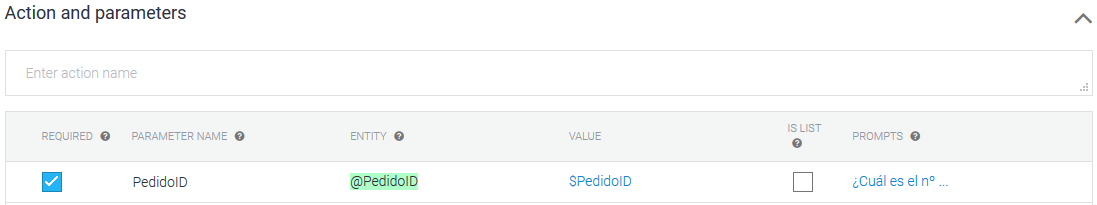
\includegraphics[width = 0.95\textwidth]{Figuras/parametersOrderID.PNG}
	\end{center}
	\caption{\label{fig:parametros} Configuración de los parámetros}
\end{figure}

Se puede indicar al agente que active un intent si se produce un determinado evento, como puede ser el caso del intent "Welcome" que se lleva a cabo cuando se abre el chat. Por ejemplo: cuando el agente no encuentra ninguna correspondencia con el registro de intents, se activa el intent "Default Fallback Intent", debido a que ha sido configurado con la entrada \textit{"input.unknown"}


Por último, es posible especificar contextos de entrada y salida que sirven para relacionar diferentes intents manteniendo información entre ellos. Cuando se produce una coincidencia con un intent, si cuenta con un contexto de salida definido se activará. Si hay contextos activos, el agente tendrá más probabilidades de establecer una coincidencia con intents que tengan definido el contexto activo como contexto de entrada. Por ejemplo: cuando se activa el intent "Buscar producto" también lo hace el contexto \textit{"Buscarproducto-followup"} que a su vez está configurado como contexto de entrada para los intents "Buscar producto - tarjetas gráficas", "Buscar producto - teclados", "Buscar producto - ratones". Por tanto, si el usuario no ha seleccionado previamente la búsqueda de un producto, entonces no se producirá una coincidencia con ninguno de estos intents. A continuación, se muestra un detalle de cómo se han configurado los contextos de entrada y salida para el intent "Buscar producto - teclados":

\begin{figure}[ht]
	\begin{center}
		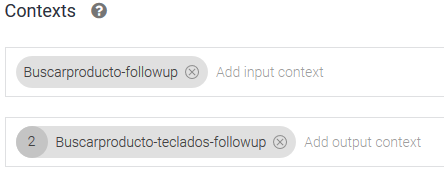
\includegraphics[width = 0.70\textwidth]{Figuras/contexts.PNG}
	\end{center}
	\caption{\label{fig:contextos} Configuración de los contextos}
\end{figure}

\newpage

\subsubsection{Entidades}

Las entidades son útiles para categorizar el contenido proporcionado por el usuario y extraer información del mismo. Dialogflow ofrece una buena cantidad de entidades predefinidas que sirven para identificar tipos de datos comunes. A pesar de ello, en este proyecto se han creado tres entidades que almacenen la información necesaria para realizar peticiones a la base de datos. Aunque actualmente el agente no está conectado a la base de datos, si que se plantea como trabajo futuro. De esta forma, se ha querido al menos sentar las bases para su posterior implementación. Las tres entidades creadas son:

\begin{itemize}
    \item \textbf{@marca}. Engloba todas las palabras para referirse a las diferentes marcas a las que pertenecen los productos que el negocio tiene en venta.
    
     \begin{figure}[ht]
    	\begin{center}
    		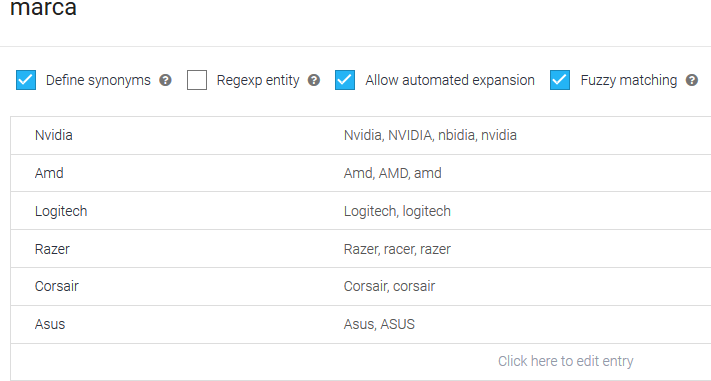
\includegraphics[width = 0.95\textwidth]{Figuras/entityMarca.PNG}
    	\end{center}
    	\caption{\label{fig:entidadMarca} Configuración de la entidad @marca}
    \end{figure}
    
    \item \textbf{@PedidoID}. Se ha definido una expresión regular para identificar los números de pedido. En este caso se trata de un número de cinco cifras comprendidas entre 0 y 9.
    
     \begin{figure}[ht]
    	\begin{center}
    		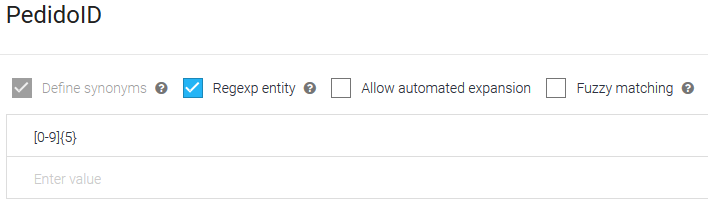
\includegraphics[width = 0.95\textwidth]{Figuras/entityPedidoID.PNG}
    	\end{center}
    	\caption{\label{fig:entidadPedido} Configuración de la entidad @PedidoID}
    \end{figure}
    
    \newpage
    
    \item \textbf{@producto}. En esta entidad se recogen los diferentes nombres con los que identificar a los productos que se venden en la página web.
    
    \begin{figure}[ht]
    	\begin{center}
    		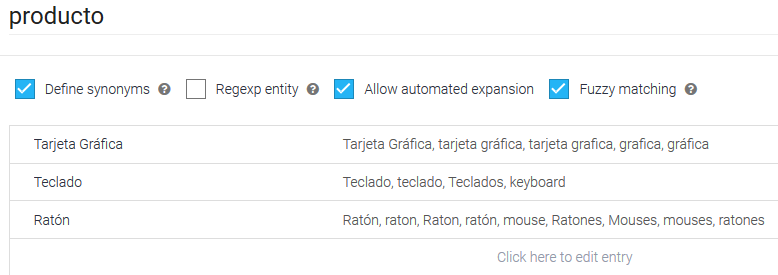
\includegraphics[width = 0.95\textwidth]{Figuras/entityProducto.PNG}
    	\end{center}
    	\caption{\label{fig:entidadProducto} Configuración de la entidad @producto}
    \end{figure}
\end{itemize}

Como se puede observar en las imágenes anteriores, para cada palabra perteneciente a una entidad se definen una serie de sinónimos que pueden ser utilizados por el usuario para referirse al mismo concepto. Además en la parte superior se encuentran las opciones "Allow automated expression" y "Fuzzy Matching". Mediante la primera opción, se activa o desactiva el aprendizaje automático del motor de lenguaje, esta capacidad permite al motor proveer nuevos sinónimos para los distintos elementos pertenecientes a la entidad. En cuanto a la segunda opción, si se activa, permite al motor extraer los parámetros que coincidan con una entidad parcialmente (en lugar de exactamente), de esta forma el motor intentará encontrar coincidencias teniendo en cuenta errores de escritura o la introducción de sólo una parte de las palabras que forman una entrada de la entidad. 

\newpage

\subsubsection{Integración}

Dialogflow se puede integrar fácilmente en un gran abanico de plataformas de conversación populares. Admite hasta 17 plataformas entre las que se encuentran Twitter, Facebook, Slack, Google Assistant, Skype, etc. También se pueden desarrollar integraciones independientes con otras plataformas haciendo uso de la API de Dialogflow, sin embargo, Google no ofrece asistencia para este tipo de integraciones.

Con el objetivo de incorporar el bot conversacional a Wordpress se ha usado MyChatbot, una extensión completamente gratuita y de instalación sencilla. Para conectar este plugin con el bot conversacional basta con copiar el token de acceso que provee Dialogflow en el campo "Access token" situado en la pestaña de configuración de MyChabot.

Dialogflow sólo permite los mensajes de respuesta enriquecida en algunas plataformas de mensajería como Slack, Skype, Facebook, etc. Con este tipo de mensajes se pueden incorporar imágenes, botones, enlaces, tarjetas, entre otras características. Por este motivo se ha desarrollado el bot usando Facebook Messenger como plataforma de mensajería. Esta decisión no supone ningún problema porque MyChatbot puede adoptar la apariencia de algunas plataformas de mensajería, simplemente dentro de las opciones de configuración se selecciona la plataforma deseada. 

En la siguiente figura se muestra cómo configurar MyChatbot:

\begin{figure}[ht]
    	\begin{center}
    		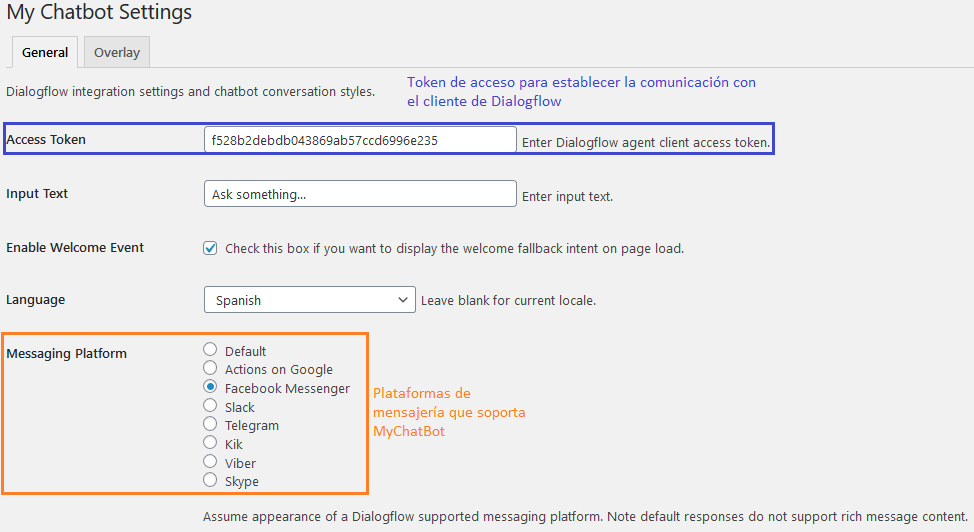
\includegraphics[width = 0.95\textwidth]{Figuras/configuracionMychatbot.png}
    	\end{center}
    	\caption{\label{fig:mychatbotConfig} Configuración del plugin MyChatbot}
\end{figure}

\newpage

\section{Despliegue}

En este sección se detalla cómo crear y desplegar los contenedores de la página web y la aplicación de análisis de sentimientos. Se dedica una subsección para explicar el proceso específico de cada proyecto, que estará estructurada de la siguiente forma:

\begin{itemize}
    \item \textbf{Modificaciones necesarias en el proyecto}. Principalmente, se deben actualizar las variables que controlan el acceso a la base de datos, debido a que se utilizará una instancia del servicio Cloud SQL. Además, en el caso de Wordpress, también se debe forzar la conexión HTTPS, ya que es el protocolo usado por Cloud Run.
    \item \textbf{Dockerfile}. Se detallará la implementación de los ficheros utilizados para la construcción de los contenedores.
    \item \textbf{Configuración del servicio en Cloud Run}. Se explicarán las opciones disponibles para configurar el servicio. Existen tres menús diferentes:
    \begin{itemize}
        \item Contenedor. Incluye las opciones de capacidad y autoescalado del contenedor, así como algunos campos generales.
        \item Variables. Aquí se establecen las variables de entorno.
        \item Conexiones. Se deben definir las conexiones de la aplicación con otros servicios de Google Cloud.
    \end{itemize}
\end{itemize}

En la siguiente imagen se muestran gráficamente los pasos que se seguirán:

\begin{figure}[ht]
    	\begin{center}
    		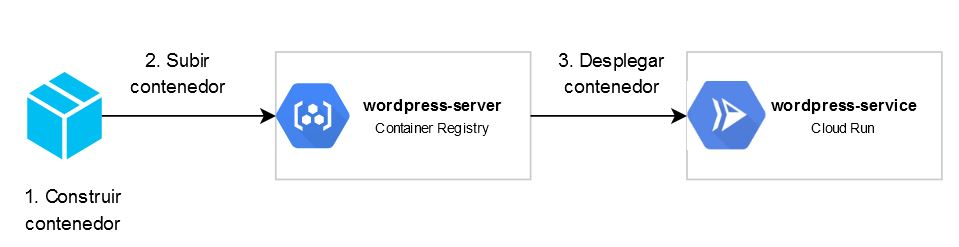
\includegraphics[width = 0.95\textwidth]{Figuras/Despliegue.JPG}
    	\end{center}
    	\caption{\label{fig:deployCloudRun} Pasos para crear un servicio en Cloud Run}
\end{figure}

Antes de proceder con el desarrollo específico de cada aplicación, el primer paso es configurar una instancia de MySQL en Cloud SQL que será necesaria para ambas aplicaciones.

\newpage

Este proceso es sencillo, una vez en el menú principal de Cloud SQL se selecciona "Crear Instancia" y se escoge el tipo MySQL. A continuación, se requiere introducir la información de la instancia que incluye un id de instancia, contraseña, ubicación, zona y versión de la base de datos. En la siguiente imagen se muestra dicha información:

\begin{figure}[ht]
    	\begin{center}
    		\includegraphics[width = 0.50\textwidth]{Figuras/informaciónCloudSQL.PNG}
    	\end{center}
    	\caption{\label{fig:informacionCloudSQL} Información de la instancia de Cloud SQL}
\end{figure}

Se presentan además una serie de opciones de configuración, escogiendo en su mayoría las opciones por defecto. Para este proyecto se ha seleccionado el tipo de máquina db-f1-micro, ya que con la opción más simple es suficiente. También se debe habilitar la IP pública para poder acceder a la base de datos desde diferentes equipos. A continuación, se enseñan ambos apartados de configuración:

\newpage

\begin{figure}[ht]
\begin{subfigure}{0.5\textwidth}
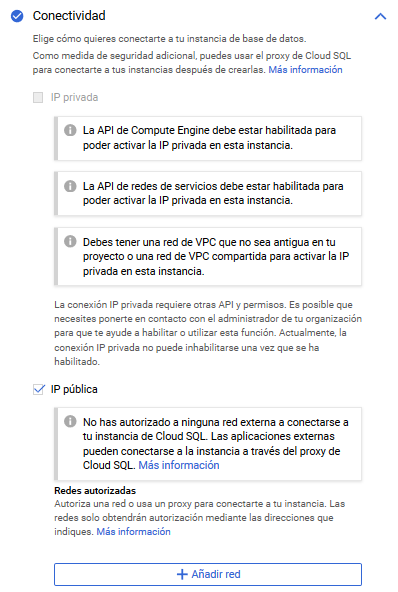
\includegraphics[width=0.9\linewidth, height=10cm]{Figuras/ConectividadSQL.PNG}
\caption{Conectividad Cloud SQL}
\label{fig:conectividadSQL}
\end{subfigure}
\begin{subfigure}{0.5\textwidth}
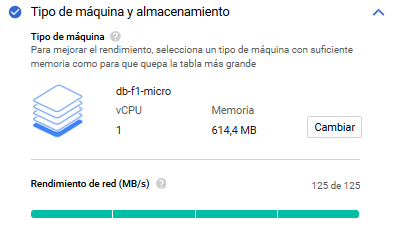
\includegraphics[width=0.9\linewidth, height=5cm]{Figuras/InstanciaCloudSQL.PNG}
\caption{Instancia Cloud SQL}
\label{fig:instanciaSQL}
\end{subfigure}

\caption{Opciones de configuración Cloud SQL}
\label{fig:configuracionCloudSQL}
\end{figure}

Una vez creada la base de datos en Cloud SQL hay que proceder a transferir los datos utilizados en el entorno local. Para ello, primero se exporta la base de datos utilizada por Wordpress desde la interfaz de phpMyAdmin. Después, haciendo uso del servicio de Cloud Storage se sube el fichero resultante de la exportación para que sea accesible al resto de servicios de Google Cloud. Por último, desde el menú "Visión General de Cloud SQL" se selecciona la opción "Importar", una vez aquí se debe elegir el archivo anterior y la base de datos donde importar la información.

\subsection{Página web}

\subsubsection{Modificaciones necesarias del proyecto local}

Como a partir de ahora se utilizará una base de datos diferente a la configurada inicialmente en local, es necesario introducir modificaciones en el archivo \textit{wp\_config}. En primer lugar se deben cambiar los campos relacionados con la conexión a la base de datos para hacer uso de variables de entorno. Sus valores se especificarán cuando se realice el despliegue del contenedor en Cloud Run.

\newpage 

\begin{lstlisting}[caption= Variables de entorno wp-config.php]
define('DB_NAME', getenv('DB_NAME'));
define('DB_USER', getenv('DB_USER'));
define('DB_PASSWORD', getenv('DB_PASSWORD'));
define('DB_HOST', getenv('DB_HOST'));
\end{lstlisting}

En segundo lugar, es necesario introducir el siguiente fragmento de código al inicio del fichero para forzar la conexión HTTPS en el área de administración (wp-admin), debido a que Cloud Run redirige todas las peticiones HTTP a HTTPS:

\begin{lstlisting}[caption= Forzar conexi\'on https]
if (
 isset($_SERVER['HTTP_X_FORWARDED_PROTO']) &&
 strpos($_SERVER['HTTP_X_FORWARDED_PROTO'], 'https') !== false
) {
 define('FORCE_SSL_ADMIN', true);
 $_SERVER['HTTPS'] = 'on';
}
\end{lstlisting}

\subsubsection{Dockerfile}

Una vez introducidas las modificaciones necesarias en los ficheros de Wordpress, se procede a crear la imagen de contenedor del proyecto que se encuentra en local. Las instrucciones para su creación se indican mediante el siguiente fichero dockerfile:

\begin{lstlisting}[caption= Dockerfile de Wordpress]
FROM wordpress:5.4.2-php7.2-apache

EXPOSE 8080

RUN sed -i 's/80/8080/g' /etc/apache2/sites-available/000-default.conf /etc/apache2/ports.conf

COPY --chown=www-data:www-data ./ /var/www/html/

WORKDIR /var/www/html/
\end{lstlisting}
 
De todas las imágenes de contenedor de Wordpress disponibles en el repositorio de docker hub, se ha seleccionado la que incluye las versiones más actualizadas de Wordpress y PHP, así como,  un servidor web que se indica mediante la etiqueta \textit{-apache}. A partir de esta imagen, se introducen algunas modificaciones para construir un contenedor propio. 

A través del comando \textit{EXPOSE 8080} se establece que éste sea el puerto de escucha utilizado por el contenedor durante su ejecución. Sin embargo, la imagen predeterminada de Apache escucha en el puerto 80, por lo tanto, se reemplaza su valor por el de 8080 utilizando el comando \textit{sed}.

Cuando la página web se encuentre en línea, su contenido será servido a través de Apache. Si se quiere introducir alguna modificación desde el panel de control de Wordpress se realizará mediante el usuario asignado a Apache, \textit{www-data}, que es diferente del usuario actual de nuestra carpeta en local. Por tanto, para evitar un error de permisos se modifica el propietario de los ficheros del proyecto en local con la instrucción \textit{--chown=www-data:www-data}. También es necesario que el contenido de la página esté disponible en el directorio de trabajo del servidor web, por ello se copia el contenido del proyecto en \textit{/var/www/html/}.

Por último, únicamente se debe establecer como directorio de trabajo el del servidor web. Esto se realiza con la instrucción \textit{WORKDIR /var/www/html/}.

Una vez que se ha creado el contenedor, el siguiente paso es subirlo a Container Registry, el servicio donde se alojan las imágenes de contenedores de forma que puedan ser usadas por el resto de servicios de Google Cloud. Los comandos que se deben ejecutar a través de la consola son los siguientes:

\begin{lstlisting}[caption= Subir imagen del contenedor a Container Registry]
docker tag <ID de la imagen> gcr.io/sentiments-analysis-263717/wordpress-server
docker push gcr.io/sentiments-analysis-263717/wordpress-server
\end{lstlisting}

donde:
\begin{itemize}
    \item gcr.io es el host de Container Registry;
    \item sentiments-analysis-263717 es el nombre del proyecto;
    \item wordpress-server es el nombre del servidor.
\end{itemize}

\subsubsection{Configuración del servicio en Cloud Run}

Tras completar esta tarea se procede a crear el servicio de Cloud Run que hará uso de dicha imagen. En primer lugar, se debe realizar la configuración del servicio indicando la región donde se ubicará el mismo, el nombre y la forma de autenticación. Es importante permitir las invocaciones sin autenticar ya que se está implementando una página web de acceso libre. La otra opción "Requerir Autenticación" hace uso de Cloud IAM, un servicio mediante el que Google permite configurar el control de acceso a través de cuentas de servicio que se utilizan para restringir las llamadas a las APIs autorizadas. 

A continuación, se pueden observar las opciones de configuración:

\begin{figure}[ht]
    	\begin{center}
    		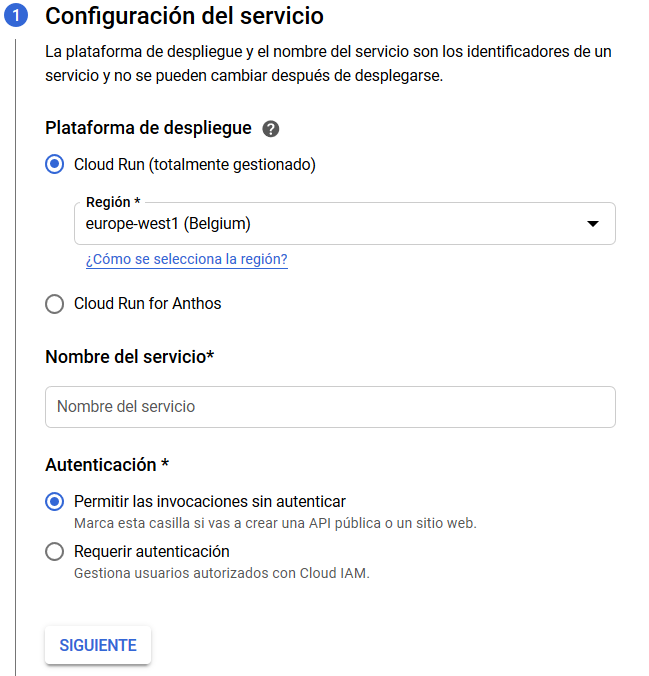
\includegraphics[width = 0.60\textwidth]{Figuras/WordpressCloudRun1.PNG}
    	\end{center}
    	\caption{\label{fig:CloudRun1} Configurar servicio de Cloud Run. Parte I}
\end{figure}

El siguiente paso consiste en configurar el contenedor desde Cloud Run. Estas opciones se encuentran en el menú de "CONTENEDOR", cada uno de sus campos está acompañado de un breve fragmento de texto explicando su función. Aquí se debe indicar el puerto de escucha del contenedor y elegir una cuenta de servicio. Además, conviene ajustar la capacidad del contenedor en función de las necesidades del servicio que se quiere desplegar.

Es necesario otorgar los siguientes roles a la cuenta de servicio que vaya a ser utilizada para ejecutar la imagen del contenedor:
\begin{itemize}
    \item Cliente de Cloud SQL. Proporciona acceso de conectividad a Cloud SQL.
    \item Agente del servicio Cloud Run. Permite que Cloud Run acceda a los recursos gestionados.
\end{itemize}

La configuración de las cuentas de servicio se realiza en el servicio Cloud IAM. Como en este caso se ha utilizado la cuenta predeterminada del proyecto cloud, se selecciona y se añaden los roles indicados anteriormente. En la siguiente figura se muestra la cuenta de servicio y sus roles:

\begin{figure}[ht]
    	\begin{center}
    		
\includegraphics[width = 0.95\textwidth]{Figuras/rolesCloudIAM.PNG}
    	\end{center}
    	\caption{\label{fig:IAM} Cuenta de servicio}
\end{figure}

Sobre la capacidad se pueden modificar los siguientes campos:
\begin{itemize}
    \item Memoria asignada. Memoria asignada a cada una de las instancias del contenedor. Acepta las unidades MiB, GiB, MB y GB.
    \item CPU asignada. Número de vCPU asignadas a cada instancia del contenedor.
    \item Tiempo de espera de solicitud. Espacio en el que espera recibir una respuesta. Se indica en segundos y el límite es de 900s.
    \item Número máximo de solicitudes por contenedor. El máximo número de peticiones que una instancia puede manejar de forma simultánea.
\end{itemize}

En cuanto al autoescalado, sólo se puede modificar el número máximo de instancias que puede crear Cloud Run en función del número de peticiones que esté recibiendo.

Seguidamente, se pueden observar los campos de configuración relacionados con la capacidad y el autoescalado:

\begin{figure}[ht]
    	\begin{center}
    		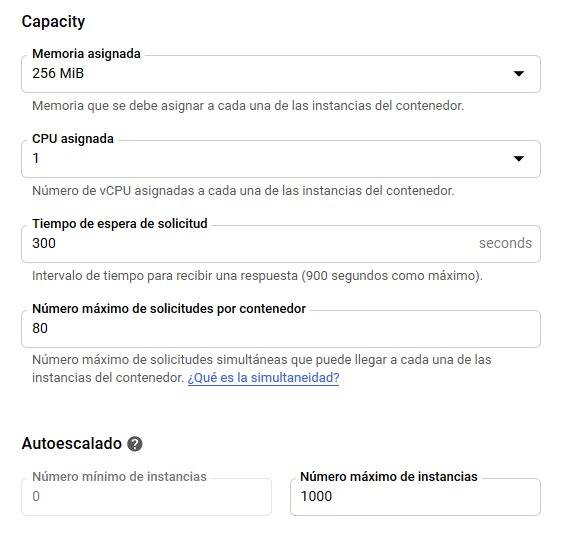
\includegraphics[width = 0.70\textwidth]{Figuras/CapacidadAutoescaladoCloudRun.PNG}
    	\end{center}
    	\caption{\label{fig:CapacidadCloudRun} Capacidad y autoescalado del contenedor en Cloud Run}
\end{figure}

\newpage

En el apartado de "VARIABLES" se deben especificar las variables de entorno utilizadas en el archivo \textit{wp\_config.php} para establecer la conexión con la base de datos. En la próxima figura se muestran las variables creadas:

\begin{figure}[ht]
    	\begin{center}
    		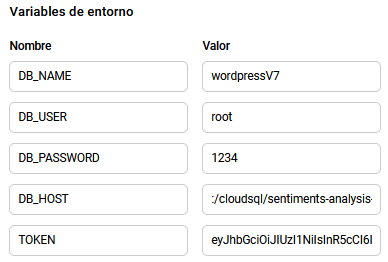
\includegraphics[width = 0.60\textwidth]{Figuras/VariablesCloudRun.PNG}
    	\end{center}
    	\caption{\label{fig:VariablesCloudRun} Variables de entorno Cloud Run}
\end{figure}

El campo DB\_HOST debe cumplir con el siguiente formato \textit{:/cloudsql/Nombre\_Conexión\_Instancia}. El valor de este parámetro puede ser encontrado en la pestaña "Visión General" de Cloud SQL, de la manera que se muestra:

\begin{figure}[ht]
    	\begin{center}
    		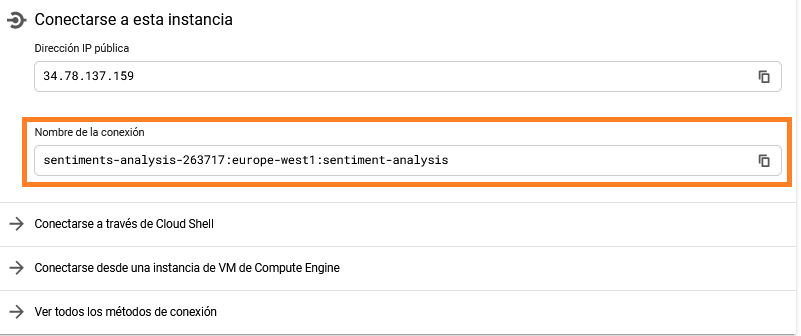
\includegraphics[width = 0.70\textwidth]{Figuras/NombreCloudSQL.PNG}
    	\end{center}
    	\caption{\label{fig:NombreCloudSQL} Nombre de conexión Cloud SQL}
\end{figure}

\newpage

Para finalizar con la configuración tan sólo falta conectar el servicio de Cloud Run con la instancia de Cloud SQL, seleccionando en el menú desplegable de la pestaña "CONEXIONES" la instancia que se va a utilizar. La próxima imagen muestra la configuración de las conexiones:

\begin{figure}[ht]
    	\begin{center}
    		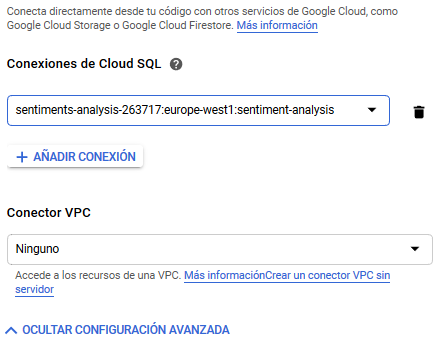
\includegraphics[width = 0.55\textwidth]{Figuras/ConexionCloudSQL.PNG}
    	\end{center}
    	\caption{\label{fig:ConexionCloudSQL} Configuración de la conexión}
\end{figure}

\newpage

\subsection{Análisis de sentimientos}

\subsubsection{Modificaciones necesarias del proyecto local}

Una vez desplegada, la aplicación utilizará la misma instancia de Cloud SQL que Wordpress. Por tanto, se debe modificar la función de la aplicación que configura la forma de acceder a la base de datos. Para ello se ha introducido una variable de entorno que comprueba si se está ejecutando la aplicación en local o producción y, en función de ella, se realiza la conexión con la base de datos de un modo u otro:

\begin{lstlisting}[caption= Conexi\'on a la BBDD en funci\'on del entorno de trabajo]
    if config.IsProduction {
		var dbURI string
		dbURI = fmt.Sprintf("%s:%s@unix(/cloudsql/%s)/%s",
			config.DBConn.DBUser, config.DBConn.DBPwd, config.DBConn.InstanceConnectionName, config.DBConn.DBName)

		dbPool, err := sql.Open("mysql", dbURI)
		if err != nil {
			panic("Failed to initialize the database")
		}

		return &Connection{Conn: dbPool}
	}

	db, err := sql.Open(config.DBConn.DBDriver,
		config.DBConn.DBUser+":"+config.DBConn.DBPwd+"@/"+config.DBConn.DBName)
	if err != nil {
		panic("Failed to initialize the database")
	}

	return &Connection{Conn: db}
\end{lstlisting}

Además, la inicialización de las variables de conexión a la BBDD también se realiza teniendo en cuenta el entorno como se puede apreciar: 

\begin{lstlisting}[caption= Inicializaci\'on de variables de conexi\'on a la BBDD]
func init() {
	if mustGetenv("PRODUCTION") == "true" {
		IsProduction = true

		Key = mustGetenv("KEY")

		DBConn.DBUser = mustGetenv("DB_USER")
		DBConn.DBPwd = mustGetenv("DB_PWD")
		DBConn.InstanceConnectionName = mustGetenv("INSTANCE_CONNECTION_NAME")
		DBConn.DBName = mustGetenv("DB_NAME")
		return
	}
	DBConn.DBUser = "root"
	DBConn.DBPwd = ""
	DBConn.DBDriver = "mysql"
	DBConn.DBName = "project"
}
\end{lstlisting}

Más adelante será necesario establecer estas variables de entorno durante la configuración del servicio en Cloud Run.

\subsubsection{Dockerfile}

Tras haber realizado las modificaciones necesarias en la aplicación, se procede con la creación del contenedor. El fichero implementado es el siguiente:

\begin{lstlisting}[caption= Dockerfile an\'alisis de sentimientos]
FROM golang:1.13

ENV PORT 5002

RUN mkdir /app
WORKDIR /app/
COPY . .

RUN go mod download && \
    go install .

CMD ["code.sentiments"]
\end{lstlisting}

Con FROM se indica la imagen base para la construcción de la aplicación dentro del contenedor que, en este caso, se trata de la última versión de Go 1.13, debido a que la aplicación utiliza esta distribución.

El contenedor utilizará el puerto 5002 para comunicarse con los clientes del servicio, que se especifica creando una variable de entorno PORT.

A continuación, se crea el directorio "/app" mediante el comando RUN  - permite ejecutar un comando SHELL en el contenedor- seguido de la instrucción unix, mkdir. Esta carpeta se establece como el directorio de trabajo del contenedor con el comando WORKDIR y se copia todo el contenido de la aplicación en él utilizando COPY.

En las siguientes líneas se actualizan las dependencias del proyecto mediante "go mod download" y se crea el ejecutable de la aplicación en el directorio actual, "go install ."

Finalmente, se ejecuta el módulo de Go que identifica la aplicación. A diferencia de RUN, el comando CMD se ejecuta una vez que el contenedor se ha inicializado, en lugar de durante la creación de la imagen. Un módulo de Go es una colección de paquetes almacenados en un árbol de archivos que tienen como raíz un fichero "go.mod" donde se definen las rutas de importación así como los requisitos de dependencia.

Una vez creado el Dockerfile se construye la imagen del contenedor y se almacena en Container Registry ejecutando las siguientes instrucciones en consola:
\begin{lstlisting}[caption= Crear y subir imagen del contenedor a Container Registry]
docker build ./
docker tag <ID de la imagen> gcr.io/sentiments-analysis-263717/sentiments-server
docker push gcr.io/sentiments-analysis-263717/sentiments-server
\end{lstlisting}

donde:
\begin{itemize}
    \item gcr.io es el host de Container Registry;
    \item sentiments-analysis-263717 es el nombre del proyecto;
    \item sentiments-server es el nombre del servidor.
\end{itemize}

\subsubsection{Configuración del servicio en Cloud Run}

El proceso a seguir es el mismo que el realizado en la sección anterior para desplegar la página web. Esta vez el puerto del contenedor será el 5002 como se indica en en el Dockerfile. También se deben crear las variables de entorno propias de esta aplicación. En la siguiente figura se muestran dichas variables

\begin{figure}[ht]
    	\begin{center}
    		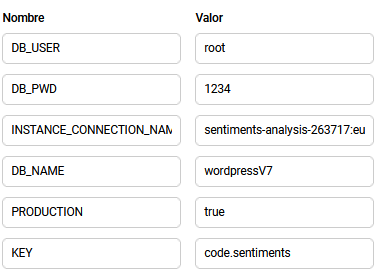
\includegraphics[width = 0.70\textwidth]{Figuras/variablesEntornoSentiments.PNG}
    	\end{center}
    	\caption{\label{fig:entornoSentiments} Variables de entorno para la aplicación de análisis de sentimientos}
\end{figure}

Tras completar la configuración, la aplicación estará disponible para su uso a partir de la URL ofrecida por Cloud Run.